\subsection{Orientation of the hand}
We want to detect the orientation of the hand in order to use training data, or detecting hand region.
In our program, major axis.py has this function.
We define the orientation of the hand as the angle of the axis of least second moment.\par
The input is the binary image of skin region.
Axis of least second moment minimizes E, the sum of the distance from all points to the line. That is,
$$E = \int \int r^2 b(x,y) dxdy$$
where $r$ is a distance from b(x,y) to the axis and b(x,y) = 1 when a pixel (x,y) belongs to the object, otherwise 0.
Let the axis be $x\sin{\theta} - y\sin{\theta} + \rho = 0$.
Distance of point (x,y) from axis is:
$$r = |x\sin{\theta}-y\cos{\theta}+\rho|$$.
Thus minimizing $E$ means minimizing
$$E = \int\int (x\sin{\theta}-y\cos{\theta}+\rho)^2 b(x,y)dxdy$$
Because $\partial E / \partial \rho = 0$, we get
$$A(x_c \sin{\theta} - y_c \cos{\theta} + \rho) = 0$$
where $A$ is an area of the object and $(x_c,y_c)$ is center of the object.
This means, the axis should pass the center point of the object.
Then, we shift the coordinate system in order to set the center point as origin.
That is, 
$x'= x - x_c, y' = y - y_c$.
Because this line should pass the origin, the line can be represented as
$x'\sin{\theta}-y'\cos{\theta}$
So, $$E = a \sin^2{\theta} - b\sin{\theta}\cos{\theta} + c\cos^2{\theta}$$.
Where $a = \int\int (x')^2 b(x,y) dx'dy', b = 2\int\int x'y' b(x,y) dx'dy', 
c = \int\int (y')^2 b(x,y)dx'dy'$.\par
Because $\partial E / \partial \theta = 0$, we get
$$(a-c)\sin{2\theta} - b\cos{2\theta} = 0$$
Also, minimizing E means the second derivative is larger than 0.
Using these information, the orientation $\theta = atan2(b,a-c)/2$.\par
Fig.\ref{fig:mom2} shows the results of orientation detection and the rotated image.
The first column is an original image.
The second column is a translated image. First, the center point of the hand moves to the center point of the image.
The light blue line is the axis. The blue dot is the center point.
For the mask, the image is rotated by the angle of $-\theta$ and translated to the original position.
The figure shows that this axis does not depends on the small fingertip movement.
If the binary image of hand has enough amount of areas, this system can detect the angle of the hand.
If the image of hand does not have enough amount of areas, for example, it can detect only a part of fingers,
it cannot detect the angle of the hand correctly.
However, because of our settings, we always can see enough amount of hand in the target area.
\begin{figure}
 \begin{tabular}{ll}
 Original image & Rotated hands \\
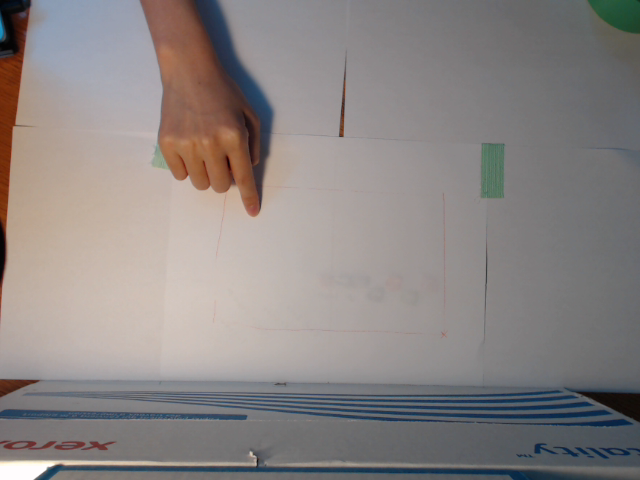
\includegraphics[width=5cm]{fig7/1-b.png} &
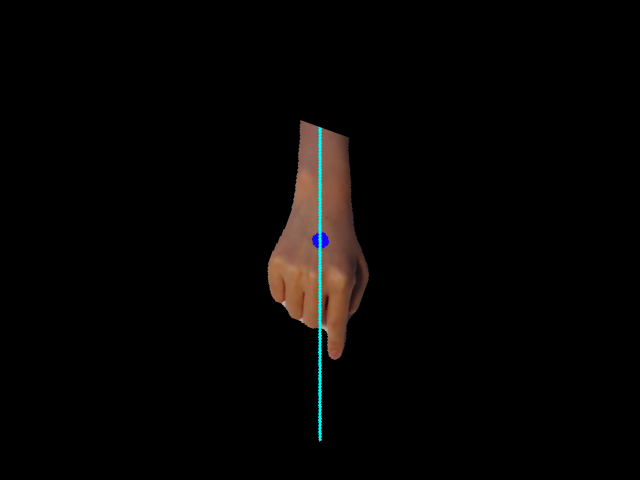
\includegraphics[width=5cm]{fig7/1-a.png} \\
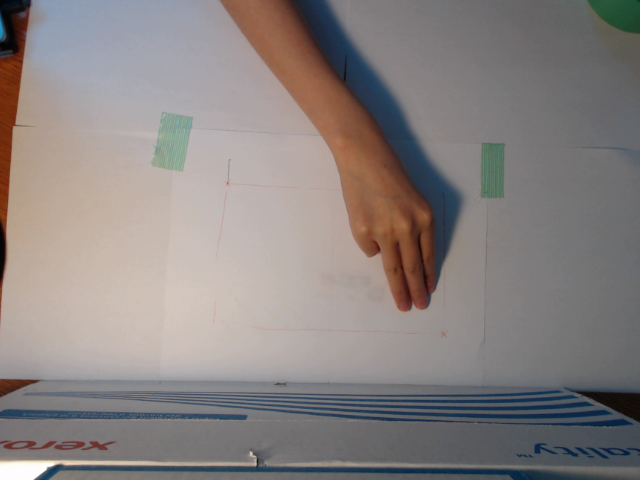
\includegraphics[width=5cm]{fig7/2-b.png} &
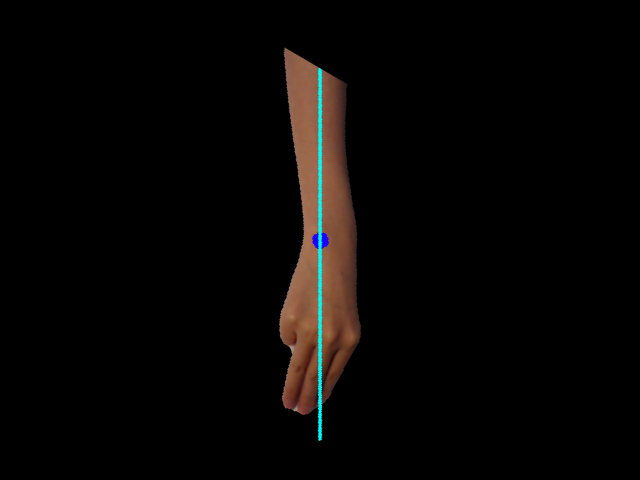
\includegraphics[width=5cm]{fig7/2-a.png} \\
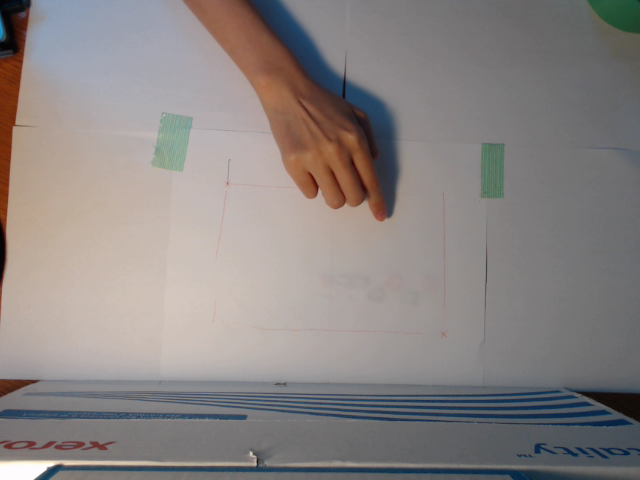
\includegraphics[width=5cm]{fig7/3-b.png} &
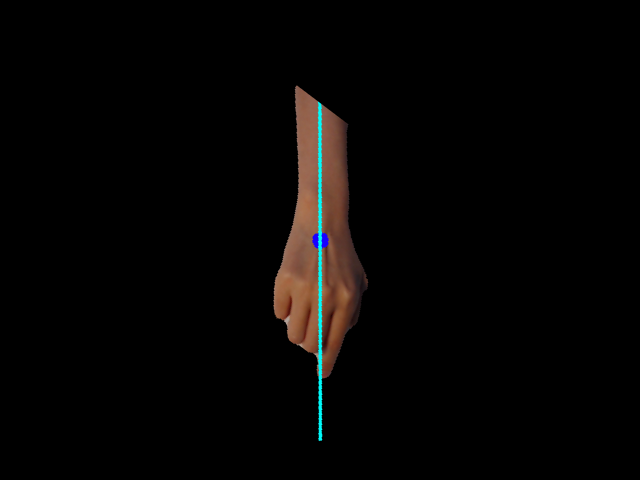
\includegraphics[width=5cm]{fig7/3-a.png} \\
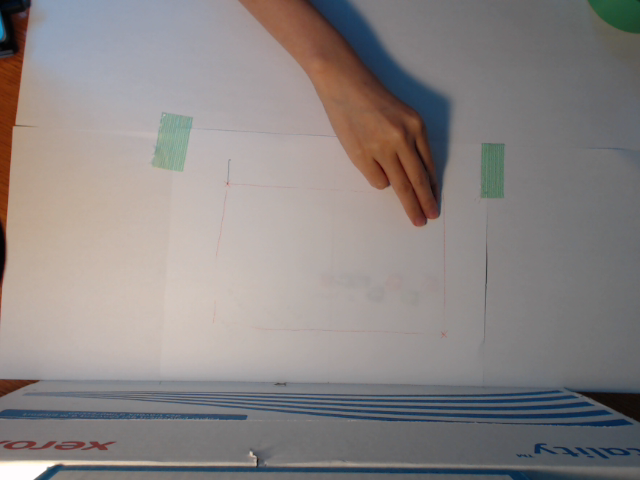
\includegraphics[width=5cm]{fig7/4-b.png} &
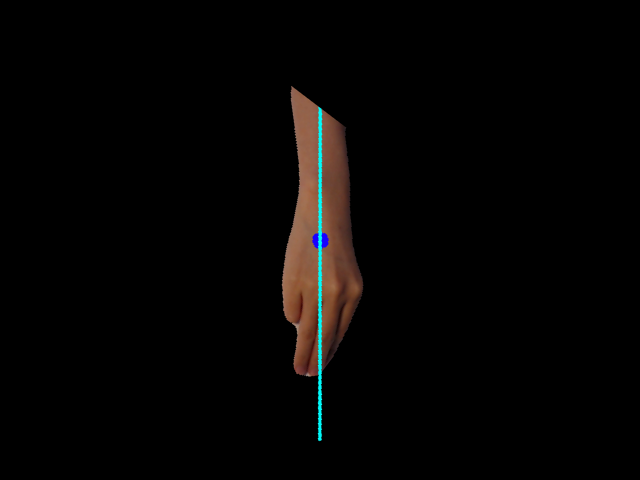
\includegraphics[width=5cm]{fig7/4-a.png} \\
\end{tabular}

 \caption{The results for orientation detection}
 \label{fig:mom2}
\end{figure}
